\section{Introduction}

There are many uses for a decentralized protocol which collects signatures of a given message from a large group of independent peers.
Such a \emph{cosigning protocol} can be used, for example, to ensure that a statement from a network authority (such as a certificate authority) has been seen and validated by a diverse group of witnesses~\cite{Syta16}.
This can protect clients from harm when the authority's secret keys are compromised and malicious actors attempt to abuse them.
The same setup can also enforce software transparency in the context of closed-source software with regular updates~\cite{Niki17}.
Here, software makers could use a cosigning protocol to protect their users from updates that introduce secret backdoors---even if, for example, the inclusion of such a backdoor is ordered by a law enforcement agency~\cite{Ford16}.

In the context of blockchains and cryptocurrencies, a cosigning protocol is a central part of the \emph{\mbox{ByzCoin}} protocol~\cite{Koko16} developed at the DEDIS~lab at EPFL.
In \mbox{ByzCoin}, a proposed block needs to be signed by a threshold number of nodes to be accepted as part of the blockchain.
One of \mbox{ByzCoin}'s main improvements over other cryptocurrencies such as Bitcoin is its low transaction confirmation latency---in the range of seconds, compared to up to an hour for Bitcoin.
To achieve a confirmation latency as low as possible, the cosigning protocol underlying ByzCoin should be fast, since a transaction is only confirmed when a block that contains it is appended to the blockchain.
The cosigning protocol must tolerate a certain number of offline or malicious nodes.
For the protocol to scale well, no single node should have to process an overwhelming amount of messages, and the size of messages should be kept low.

The aim of this semester project is to design and evaluate a gossip protocol for building collective signatures.
An existing cosigning protocol built at the DEDIS~lab, \emph{BLS~CoSi}~\cite{Blscosi}, is used as a starting point.
BLS~CoSi uses the Boneh-Lynn-Shacham signature scheme~\cite{Boneh01}, which supports \emph{multi-signatures}~\cite{Boneh03}.
Multi-signatures are short signatures that can be used to verify that a large number of parties signed a common message.
To reduce the amount of data transferred and stored, this project's new cosigning protocol uses a multi-signature scheme based on BLS signatures, shown recently by Boneh, Drijvers and Neven~\cite{Boneh18}.
The existing BLS~CoSi implementation does not always handle faults in a small number of nodes well, and so there is room for improvement.
A gossip protocol is well-suited for the task of improving fault tolerance.
This report presents the new cosigning protocol and then analyzes it based on an experimental evaluation.

The main goal of the new protocol is to improve fault tolerance compared to the existing BLS~CoSi protocol while still being fast and not overwhelming any participating node.
A secondary aim is efficiency: the number of messages exchanged and the amount of data transferred between nodes should remain low.
The new protocol is designed mainly for the use case of \mbox{ByzCoin}, although other applications are certainly possible.

Section~\ref{background} of this report gives a little background on gossip protocols and the cryptographic tools used in the new cosigning protocol, and outlines the how BLS~CoSi works.
Section~\ref{implementation} presents the new gossip protocol's design and implementation.
In Section~\ref{methodology}, the methodology and setup used in the experiments is shown.
Their results are given in Section~\ref{results}.
Section~\ref{discussion} discusses the findings and limitations, and gives an outlook on future work, after which the report ends with a short conclusion in Section~\ref{conclusion}.


\section{Background}
\label{background}

The main conceptual tools used in this project are gossip protocols and the BLS cryptographic scheme along with its extensions.
The existing BLS~CoSi protocol, which we aim to replace, uses BLS cryptography, but not gossip protocols.


\subsection{Gossip protocols}
\label{gossip}

Gossip protocols can be used for a range of tasks where information needs to be shared between different nodes.
Among other things, they are used for information dissemination and computing an aggregate between many nodes~\cite{Birm07}.
They provide many useful properties at a reasonable efficiency.
One important such property is logarithmic \emph{mixing time}: if the number of nodes is $n$, a correctly designed gossip protocol propagates a new piece of information to all peers in $O(log(n))$ time, assuming nodes are not overwhelmed by the rate of information transfer~\cite{Birm07}.
At the same time, the number of messages that a single node sends and receives is constant in the number of peers.
Another advantage is gossip protocols' simplicity: all participating nodes can often run the same code.

A typical basic gossip protocol repeatedly runs three steps in a loop: \emph{peer selection}, \emph{data exchange} and \emph{data processing}~\cite{Kerm07}.
In the first step, peer selection, a node chooses one or more peers to exchange information with, typically at random.
Choosing a new set of random peers each time is a simple and effective way of achieving fault tolerance.

In the second step, data exchange, data is sent to or received from the selected peers.
In a \emph{push model}, information is sent to the peer and no reply is expected.
In a \emph{pull model}, a request is sent, to which the peer responds with known information.
Is is also possible to combine the two models in one protocol.

In the third (optional) step, the new information is processed or passed to a further-up application layer.
How processing is done depends on the domain and application of the protocol.

A gossip protocol that is concerned with information dissemination can be analyzed by looking at the different states in which a node can find itself in regards to an update~\cite{Jela13}.
An update is here a piece of information that is being spread.
There are usually up to three states called \emph{susceptible~(S)}, meaning the node does not know about the update, \emph{infected~(I)}, meaning the node is actively spreading the update, and \emph{removed~(R)}, meaning the node knows about the update, but is not actively spreading it (anymore).
In the SI~model, a node starts in state~S and switches to state~I when it learns about an update, after which it can no longer change its state with regards to this update.
In the SIR~model, a change to state~R is possible after the node takes on state~I.

Gossip protocols are typically long-running protocols, but in this project, we employ a very short-running protocol.
A protocol instance is started when a node makes a request for a message to be signed.
When the requesting node has received enough signatures, the protocol has fulfilled its task.
In our setup, every node knows and can exchange messages with every other node.
The set of nodes does not change during the course of a protocol instance.
These properties as well as our specific requirements affect our protocol design.

Our protocol sends push messages in a very short interval to allow signatures to be spread very quickly.
We use the SI~model because we value the speed that is gained from continuing to spread signatures pro-actively throughout the protocol's lifetime.
We use only push messages during the main part of the protocol.
Pull messages are not necessary to guarantee complete dissemination in the SI~model.
Although they have some advantages over push messages, they also have the disadvantage that its takes a full roundtrip to spread a piece of information after sending a pull message, compared to half a roundtrip for a push message.


\subsection{Multi-signatures}

A \emph{digital signature} is a tool of public-key cryptography, computed from a message and a private key, that be verified using the corresponding public key and the message.
\emph{Cosigning} or collective signing, as used in this report, means that multiple nodes digitally sign the same message or statement.
A \emph{multi-signature} is a compact value that proves that multiple nodes have signed the same message~\cite{Boneh18}.
It is computed by aggregating multiple signatures from different nodes.
The advantage of a multi-signature over a simple list of signatures from different nodes is that a multi-signature is smaller.
This is especially important in protocols where many cosignatures are exchanged between nodes, as is the case in ByzCoin~\cite{Koko16}.

The multi-signature scheme used in the new protocol is based on work by Boneh, Drijvers and Neven~\cite{Boneh18} and implemented under the name \emph{BDN} in the cryptographic library \emph{Kyber}~\cite{Kyber}.
BDN multi-signatures are based on the Boneh-Lynn-Shacham (\emph{BLS}) signature scheme~\cite{Boneh01} and use commutative groups of prime order both for signatures and for public keys.
In the version of the BDN scheme that is applied in the new cosigning protocol, the public keys of all nodes have to be known in advance, even if not all of them end up signing the message.
The public keys are used collectively to create a unique integer coefficient for each signatory: $\alpha_1$ for the first node, $\alpha_2$ for the second, and so on.
In a set of three nodes signing the same message, where $S_i$ is the signature of node~$i$, the multi-signature~$S$ is then computed as $S = \alpha_1 * S_1 + \alpha_2 * S_2 + \alpha_3 * S_3$ (using additive group notation).
A multi-signature from just part of the nodes, such as $\alpha_1 * S_1 + \alpha_3 * S_3$, is equally possible.
Thanks to commutativity and associativity, partial multi-signatures from two or more disjoint sets of peers can be added to form a new valid multi-signature.
A more in-depth explanation of the BDN scheme is found in the paper presenting the scheme~\cite{Boneh18} or an article by Snigirev~\cite{Snig18}.

To verify a multi-signature, the verifier must know the public keys of all the nodes that are part of the group, including those who did not end up signing.
This is not a problem in the context of the new cosigning protocol, as all nodes know the public keys of all peers.
The verifier must also know which nodes contributed to a multi-signature.
This is solved by storing a bitmap together with each multi-signature that indicates the contributing nodes.


\subsection{The pre-existing BLS~CoSi protocol}

In BLS~CoSi~\cite{Blscosi}, a protocol instance is initiated when a cosignature is requested on some node by a client from a higher application layer.
Authenticated communication with other nodes is handled by the \emph{Cothority} framework~\cite{Coth} which BLS~CoSi is a part of, as is the distribution of public keys and membership of nodes.
It can therefore be assumed that all nodes know all public keys from the start and that the set of peers is known and constant for the duration of the protocol.

Generally, there is a certain threshold of nodes that must sign a message it before it is considered a valid cosignature.
In this report, we assume \emph{Byzantine consensus} is needed, which means we assume that up to $f$ out of $n = 3f+1$ nodes may be faulty (this includes offline or malicious nodes) and we require $2f+1$ nodes, i.e.~just above two thirds of nodes, to sign a message~\cite{Koko16}.

BLS~CoSi works by arranging all participating nodes in a tree of depth~3.
The root of this tree is the node where the protocol instance is initiated, which is simultaneously the node where the cosignature needs to be returned to an application layer in the end.
An initial signature request containing the message to be signed is sent by the root to all its child nodes in the tree.
These nodes then send a signature request to their children, which are leaf nodes.
The leaf nodes reply by sending their signature to their parent nodes, who then aggregate the received signatures.
They add their own signature and return the aggregated signature to the root, who then combines the aggregates and its own signature to form the final cosignature.
Of course, each node can also choose not to sign the message.
In that case, it sends a refusal message instead of a signature.

If a child of the root is faulty and does not return a proper aggregate, the root potentially misses out on a lot of signatures.
To mitigate this problem, the root rearranges the tree and tries again if, for example, it has not heard back from a child after a few seconds.
This solution is not ideal, however, as it is possible that multiple attempts are needed, which can cost a lot of time.


\section{The new protocol's design and implementation}
\label{implementation}

Like the old BLS~CoSi implementation, the new cosigning protocol is written in Go and fits into the Cothority project~\cite{Coth}.
It makes use of different tools developed by the DEDIS lab, including Kyber~\cite{Kyber}.

The interface for calling the new protocol is the same as for BLS~CoSi.
As before, the protocol starts with a single node, the \emph{root}, needing a cosignature.
Any node can start a protocol instance and will then be the root for this instance.
The root has a special role in the protocol, as the root needs to return a cosignature to an application layer in the end.


\subsection{Rumor messages}

During the main part of the protocol, only one type of message is exchanged between nodes, called a \emph{rumor message}.
It contains the statement to be signed as well as all the signatures the sender has seen so far.
Of course, at the moment the protocol starts, only the root knows about the protocol.
The other nodes start participating after they receive a rumor message for the first time.

The behavior of each node during this initial phase of the protocol is simple.
After receiving a rumor message for the first time, the node adds its own signature to its collection of known signatures (assuming that the node chooses to sign the statement).
A node also adds all signatures to its collection when they are received for the first time.
Each node periodically sends a rumor message, containing the full collection of known signatures, to a set of $r$ different randomly selected peers ($r$ is smaller than the number of nodes~$n$).
This sending of rumor messages happens at a regular interval~$t$, typically a fraction of a second in a context like ByzCoin.
The parameters $r$ and~$t$ have the same fixed value for all nodes.


\subsection{Shutdown mode}

As soon as the root node has received a threshold number of signatures through this process of gossip, it sends an aggregated cosignature to the application that requested it.
At this point, the protocol has fulfilled its task, and all that is left to be done is to wind down the protocol.
This needs to be done with some care; after all, the other nodes do not know when the protocol is done.
To signal that the protocol is finished, the root sends a \emph{shutdown message} to $s$ different randomly selected peers and enters \emph{shutdown mode}, where $s$ is another parameter with the same fixed value for all nodes.
In shutdown mode, incoming rumors are answered with a shutdown message and incoming shutdown messages are ignored.
The stored collection of signatures is no longer needed in shutdown mode.
When a node receives a valid shutdown message, it sends the message on to $s$ different randomly selected peers and enters shutdown mode.
Invalid messages are simply ignored.

After the root has built a cosignature, all nodes should enter shutdown mode relatively quickly.
However, nodes generally do not know the state of other nodes, and so they remain in shutdown mode, listening for rumor messages and responding with a shutdown message, for a while longer.
This is to ensure that all nodes enter shutdown mode eventually and can cease sending out rumor messages.
After a fixed amount of time, long enough to not interfere with the course of the protocol, the node stops running the protocol.

To prevent an attack where a malicious node causes other nodes to enter shutdown mode prematurely, shutdown messages have to be signed by the root.
(The root, as the node where the signature request originates, can be assumed to be correct.)
In order to prevent a replay attack where a malicious node resends a shutdown message from a previous protocol instance signed by the same root node, the signed shutdown message needs to be unique to a protocol instance.
For this reason, we chose to use the aggregated cosignature in the shutdown message: the shutdown message contains the original statement to be signed, a valid cosignature of this statement, and a signature of the cosignature by the root.


\subsection{Signature aggregation}
\label{aggregation}

The simplest way of handling signature aggregation is to let the root to it only when it has received the threshold number of signatures.
Indeed, this was one of the variants we implemented.
However, less data needs to be transferred if signatures are aggregated sooner in the protocol.
Aggregating signatures sooner is tricky because signatures can only be aggregated if they come from disjoint sets of signatories.
For example, a multi-signature from the set of signatories $\{A, B\}$ can be aggregated with the signature of node~$C$.
However, if we try to aggregate two multi-signatures from signatories $\{A, B\}$ and $\{B, C\}$, we run into a problem because the sets of nodes are not disjoint.
Without additional information, we cannot validly aggregate these multi-signatures.

To avoid this problem while still allowing some level of early aggregation, signatures can be aggregated along a conceptual binary tree.
Each leaf in this tree stands for a signature from a single signatory.
All other nodes in the binary tree stand for the aggregation of their children.
For example, with four potential signatories $A$, $B$, $C$ and~$D$, there are four leaves, one for each of them.
One level up, we might have one parent for the aggregation $\{A, B\}$ and one for $\{C, D\}$.
At the top of the binary tree is the aggregation of these two: $\{A, B, C, D\}$.
The second protocol variant we implemented aggregates signatures if and only if the aggregation exists in this binary tree.
This way, there are never any two multi-signatures from disjoint sets of signatories.


\subsection{Further details}

In gossip protocol terminology, the rumor messages act as push messages most of the time.
However, when they reach a node in shutdown mode, they act more like a pull message, pulling the shutdown message.

The protocol is designed to spread information quickly, with efficiency only being a secondary concern.
This is why entering shutdown mode is only possible after it has been proven that the root has received a cosignature.

The parameters $r$, $s$ and $t$ are sent along with rumor messages in our current implementation to help us test the effects of these parameters in experiments.
In a real-world implementation, they would be fixed in advance.


\section{Methodology for experimentally evaluating the protocol}
\label{methodology}

To evaluate the new protocol, it was tested in simulations and compared to BLS~CoSi under varying conditions.
These conditions include the number of nodes, the number of failing nodes, and an artificial message delay, which is used to simulate real-world network delays.
The delay for any given message was randomly picked from a uniform distribution between a fixed minimum and maximum delay.
A failing node, in our simulations, drops all incoming messages and sends no messages, effectively causing the node to be offline.
If a node is not failing, it is \emph{active} and functions correctly.
The root was active in all simulations.
All experiments were run on single machine with eight 3.10~GHz Intel Core~i7 processors under Ubuntu~18.10.

Three metrics were used to evaluate the protocols.
The most important metric is the time it takes until the root returns the cosignature, called the \emph{protocol duration}.
The other two metrics we measured are the number of messages sent per active node and the amount of data sent per active node.
Both rumor messages and shutdown messages are included in these metrics.

Altogether, ten sets of simulations were run.
Each set of simulations varied one or two parameters to isolate their effect and analyze their influence.
The other parameters were set to default values.
The parameters come in two groups: environment parameters that are not within the nodes' control, and protocol parameters that affect how the nodes behave.

\subsection{Default parameter values in simulations}
\label{defaults}

The default values for environment parameters are as follows.

\begin{itemize}
    \item Number of nodes: $n = 25$
    \item Number of failing nodes: $0$
    \item Minimum message delay: $0.095$~seconds
    \item Maximum message delay: $0.105$~seconds
\end{itemize}

It follows that the mean message delay is $0.1$~seconds by default.
The small range of possible delays ($0.01$~seconds between the minimum and maximum delay) is specified to prevent unnatural effects where, for example, messages from different nodes always arrive at the same time.

The threshold of signatories for a valid cosignature is always set to $n - \lfloor \frac{n-1}{3} \rfloor$ because this is the value that is used in ByzCoin.
The default values for the other protocol parameters are as follows.

\begin{itemize}
    \item Number of recipients for each rumor message: $r = 3$
    \item Interval between sending out rumor messages: $t = 0.07$~seconds
    \item Number of initial shutdown-message recipients: $s = 2$
    \item Early aggregation along a binary tree: on
\end{itemize}

These default values for protocol parameters were chosen as a compromise between protocol speed and efficiency.


\section{Results}
\label{results}

Whenever a parameter is not mentioned in the description of an experiment, it takes on the default value given in Subsection~\ref{defaults}.

\subsection{Comparison of BLS~CoSi and the new gossip protocol}

In an initial experiment, the new gossip protocol was compared to BLS~CoSi with varying numbers of nodes and failing nodes.
We found that BLS~CoSi sometimes fails when the number of active nodes was close to the threshold of signatories (but still high enough that the threshold can be reached).
This happens when no valid signature is produced after four tries.
In the most extreme case in our experiments, with $n = 36$ and 11~failing nodes, BLS~CoSi failed 52\% of the time.

Even when it did not fail, BLS~CoSi often took many times longer to produce a cosignature than the gossip protocol, depending on the number of retries it needed.
The duration of the gossip protocol was fairly stable, always measuring in below 1.3~seconds in this set of experiments.
With very few failing nodes, however, BLS~CoSi was consistently faster than the gossip protocol.
The timings are shown for $n = 36$ in Figure~\ref{fig1time}.

\begin{figure}[!htbp]
    \centering
    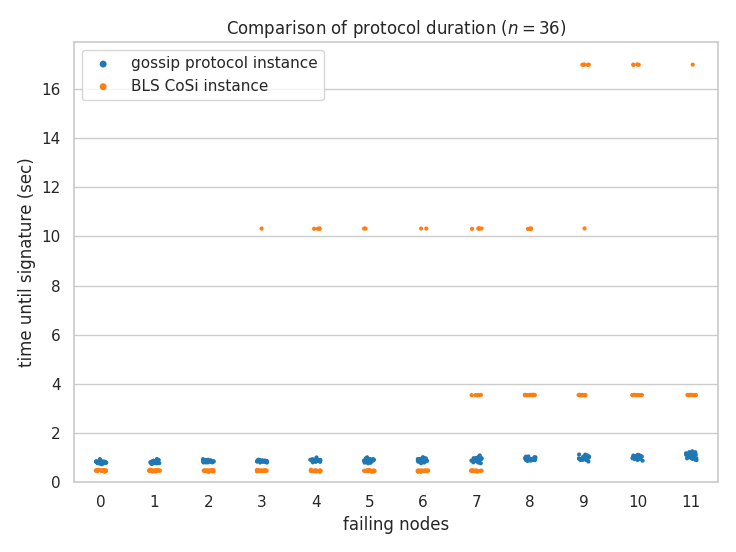
\includegraphics[width=0.95\textwidth]{figures/1/round_wall_sum_36_big.png}
    \caption{Timings until a cosignature was returned using BLS~CoSi versus the new gossip protocol. Each dot stands for a single protocol instance.}
    \label{fig1time}
\end{figure}

In the amount of data sent per active node, the gossip protocol performs slightly worse than BLS~CoSi for $n = 36$.
Still, the amount of data sent by the gossip protocol is usually less than 170\% of that sent by BLS~CoSi, as Figure~\ref{fig1data} shows.
The message count is typically around 300\% higher for the gossip protocol than for BLS~CoSi.
See Appendix~\ref{axresults} for more detailed results.

\begin{figure}[!htbp]
    \centering
    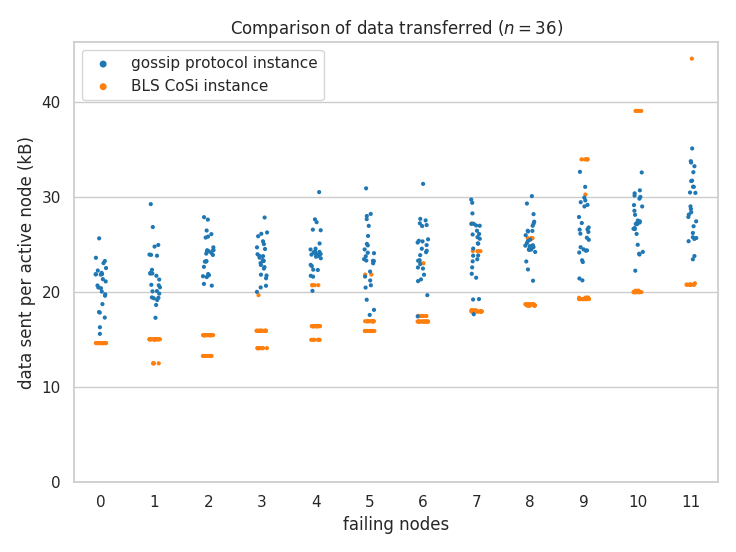
\includegraphics[width=0.95\textwidth]{figures/1/bandwidth_tx_sum_36_big.png}
    \caption{Amounts of data transferred per active node using BLS~CoSi versus the new gossip protocol}
    \label{fig1data}
\end{figure}


\subsection{The new gossip protocol under varying conditions}

A range of experiments were conducted to analyze the effects of environment parameters and protocol parameters.
In these experiments, the protocol was run multiple times under each set of parameter values, typically around 20~times.
We report and plot the mean of the measurements for these runs.

The effect of the message delay on the protocol duration is shown in Figure~\ref{fig2time}.
In this experiment, the protocol was run with different mean message delays ranging from 0.0~to 0.4~seconds.
The minimum and maximum delay are always 0.01~seconds apart (except for the special case where the minimum and maximum delay are 0.0~seconds).
The plot shows that the mean protocol duration is highly dependent on the mean message delay and that there is an approximately linear relationship between message delay and protocol duration.

\begin{figure}[!htbp]
    \centering
    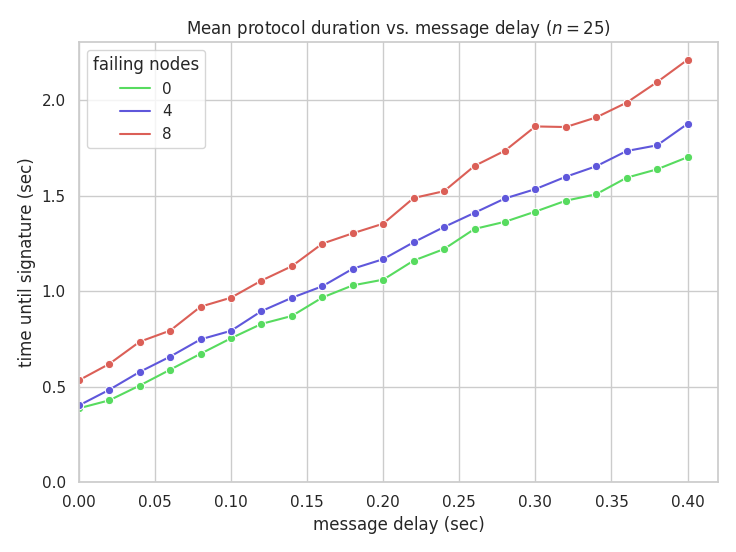
\includegraphics[width=0.95\textwidth]{figures/2/round_wall_sum_by_delay.png}
    \caption{Timings until a cosignature was returned under varying mean message delays and failing node counts}
    \label{fig2time}
\end{figure}

The experiment was run for different numbers of failing nodes.
Figure~\ref{fig2time} shows that the mean protocol duration is consistently slightly higher for higher numbers of failing nodes.
A similar roughly linear relationship was also observed for both the number of messages and the amount of data sent per active node.
This is expected, because the number of messages sent per unit of time per node is constant while the node is sending rumor messages.
Therefore, the longer a protocol takes to complete, the more messages each node is expected to send.
A plot showing the number of messages sent under these varying conditions is given in Figure~\ref{fig2msg}.

\begin{figure}[!htbp]
    \centering
    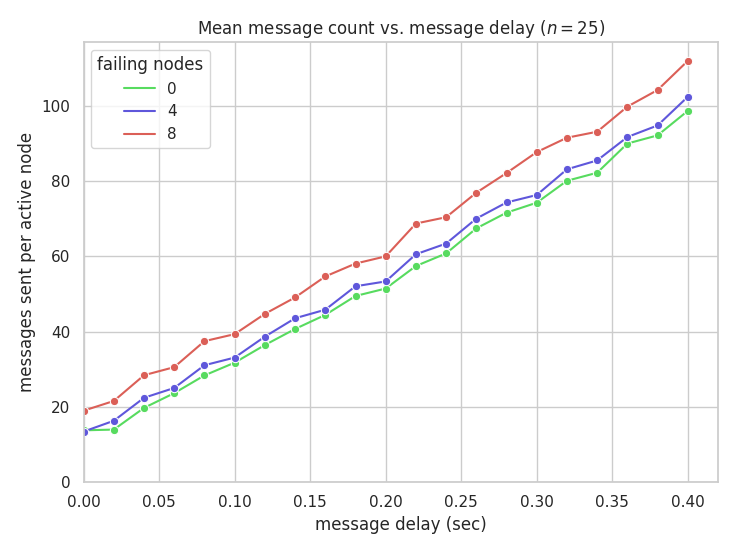
\includegraphics[width=0.95\textwidth]{figures/2/bandwidth_msg_tx_sum_by_delay_big.png}
    \caption{Number of messages sent per active node under varying mean message delays and failing node counts}
    \label{fig2msg}
\end{figure}

\begin{figure}[!htbp]
    \centering
    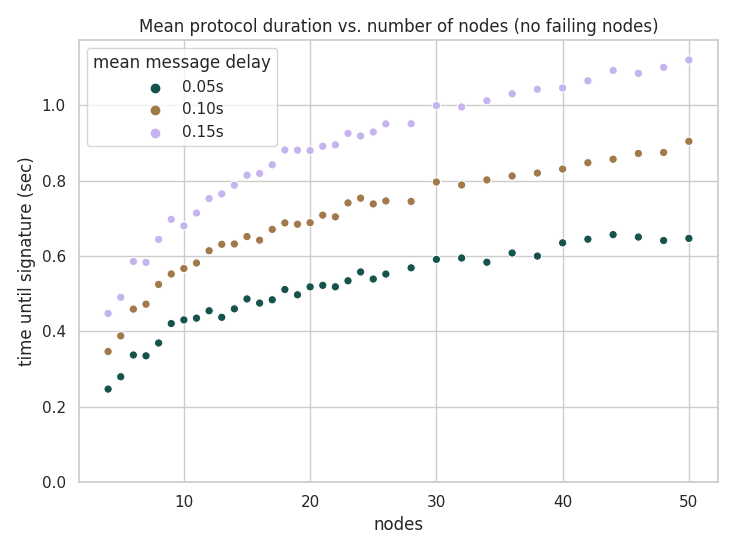
\includegraphics[width=0.95\textwidth]{figures/5/round_wall_sum_by_num_nodes.png}
    \caption{Timings until a cosignature was returned under varying mean message delays and node counts}
    \label{fig5time}
\end{figure}

The number of nodes also affects the protocol duration, as shown in Figure~\ref{fig5time}.
We can see that the number of nodes has a similar importance as the mean message delay in its effects on protocol duration.
The protocol duration grows approximately as $O(log(n))$ as predicted by the theory of gossip protocols described in Subsection~\ref{gossip}.
With $n = 50$ and a relatively pessimistic mean network delay of $0.15$~seconds, the mean protocol duration is around 1.1~seconds.

As described in Subsection~\ref{aggregation}, the new protocol can run in two modes when it comes to signature aggregation: either there is no early aggregation, or tree-based aggregation.
Figure~\ref{fig4data} shows that tree-based aggregation causes a substantial improvement in the amount of data sent per active node.
The advantage of this early aggregation is bigger the more nodes there are, with tree-based aggregation saving more than 50\% in data transferred for $n = 50$.
The aggregation setting had no observable effect on either the protocol duration or the number of messages sent.
This is expected, because the setting only affects how the transferred data is represented and does not affect the gossip protocol otherwise.

\begin{figure}[!htbp]
    \centering
    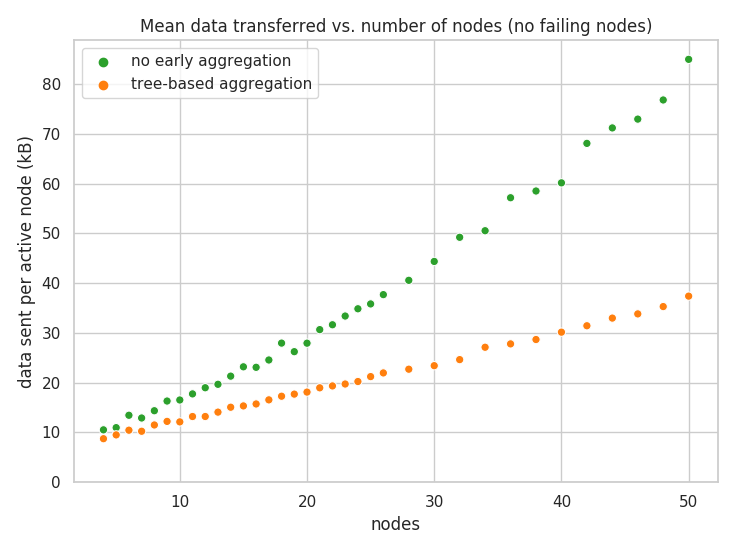
\includegraphics[width=0.95\textwidth]{figures/4/bandwidth_tx_sum_by_mode_big.png}
    \caption{Amounts of data transferred per active node under varying node counts and aggregation settings}
    \label{fig4data}
\end{figure}

\begin{figure}[!htbp]
    \centering
    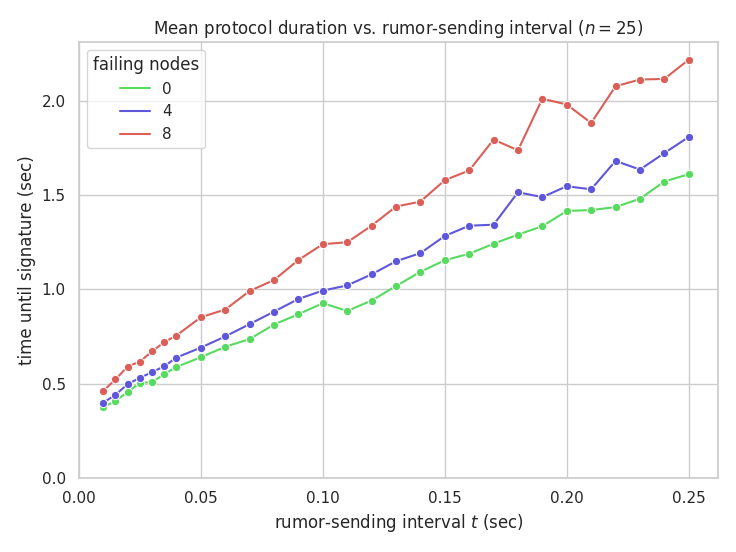
\includegraphics[width=0.95\textwidth]{figures/6/round_wall_sum_by_gossip_tick.png}
    \caption{Timings until a cosignature was returned under varying rumor-sending intervals and failing node counts}
    \label{fig6time}
\end{figure}

\begin{figure}[!htbp]
    \centering
    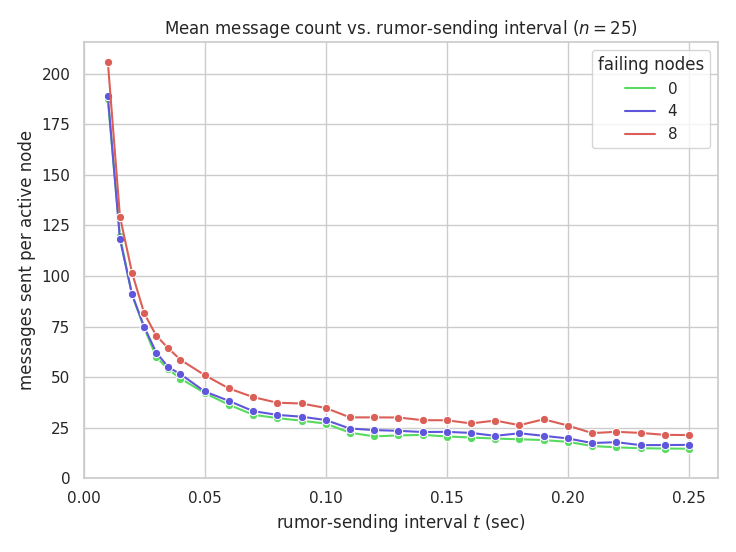
\includegraphics[width=0.95\textwidth]{figures/6/bandwidth_msg_tx_sum_by_gossip_tick_big.png}
    \caption{Number of messages sent per active node under varying rumor-sending intervals and failing node counts}
    \label{fig6msg}
\end{figure}

Another important parameter is the rumor-sending interval~$t$.
Figure~\ref{fig6time} shows that the protocol duration grows roughly linearly as a function of the rumor-sending interval.
However, the number of messages sent and the amount of data transmitted skyrocket as the rumor-sending interval tends towards zero.
For the message, this is shown in Figure~\ref{fig6msg}.
Therefore, there is a trade-off in the choice of rumor-sending interval: a shorter interval decreases the protocol duration, but increases the number of messages and the amount of data transferred.

Some more experiments were run to test the effects of other less important parameters.
Their results in the form of plots are found in Appendix~\ref{axresults} and will be summarized here.
We found that the important quantity in the aforementioned trade-off is the number of rumor messages sent per node per second.
This quantity depends on two parameters: the number of recipients for each rumor message~$r$, and the rumor-sending interval~$t$.
The number of rumor messages sent per node per second is $\frac{r}{t}$.
If the ratio between $r$ and $t$ is not changed, we found that the mean of the measured metric only varies slightly.
Changing $r$ therefore has a similar effect as changing $t$ in the opposite direction.
With $\frac{r}{t}$ constant, we found that the protocol duration is slightly lower when $r$ is reduced.
The effect is rather small and the difference between $r = 1$, $r = 2$ and $r = 3$ is hardly noticeable in our monitored metrics.

The number of initial shutdown-message recipients~$s$ had a small, but noticeable effect on the number of messages sent per active node: the total message count increases with $s$.
We do not have enough data to tell what effect $s$ has on the amount of data transferred.
As expected, $s$ has no effect on the protocol duration.

Finally, we also tested the effect of the variance in message delays on our metrics (with the mean message delay fixed at 0.1~seconds).
We found that the variance has no big impact on the three metrics we monitor.
A higher variance slightly reduced the mean protocol duration in our experiments.


\section{Analysis and discussion of the findings}
\label{discussion}

The initial goal of improving fault tolerance over BLS~CoSi is met by the new gossip cosigning protocol.
The protocol takes a reasonably short time to produce a cosignature, although an even shorter duration may be desirable for some applications.
Extreme outliers in the protocol duration almost never occur, which is an important property for many applications.
Both the number of messages exchanged and the amount of data transferred are higher than with BLS~CoSi.
This is to be expected, as the redundancy inherent to gossip protocols is avoided in BLS~CoSi.
BLS~CoSi also uses a lot more bandwidth on some nodes than on others.
Taking these considerations into account, the higher measurements for the gossip protocol on these two metrics are reasonable.
The amount of data transferred has been kept low through the optimization of aggregating signatures early.
We have experimentally backed up some predictions of gossip protocol theory (as applied to this protocol), notably that the protocol duration grows roughly like $O(log(n))$ as a function of the number of nodes $n$.


\subsection{Limitations}

The new gossip protocol still has its limitations.
It does not adapt to the properties of the network, such as the network message delay.
Ideally, a gossip protocol would send fewer messages per second in a slower network.
The rumor messages sent in the network can get quite large, depending on the number of nodes.
This has not been a problem in our experiments with up to 50~nodes, but it could easily become a problem with thousands of nodes.

Due to the inherent randomness in the gossip protocol and the unpredictability of network message delays, there is no certain upper limit for the protocol duration.
Membership needs to be closed for the duration of the protocol, and all nodes need to know each other's identities and public keys.
To be safe against man-in-the-middle attacks, the protocol needs authenticated channels for messages.


\subsection{Future work}

The gossip protocol can be improved in a number of ways.
Currently, the recipients of rumor messages are selected randomly at uniform, but there may be better ways of selecting peers.
If this is changed, care needs to be taken not to introduce new vulnerabilities into the protocol.

The current strategy of aggregating signatures along a binary tree is relatively simple and shows some clear improvements over the alternative approach of not aggregating signatures until the end.
It is possible that there are better ways of aggregating signatures.
However, this is not straightforward because signatures cannot be aggregated if the sets of signatories are not disjoint.

The current implementation relies solely on push messages to construct a cosignature.
Adding pull messages may be an improvement.
For example, nodes might specifically pull from peers whose signature they are missing.

The protocol's properties have not been formally proven.
This could become necessary if, for example, the statistical properties of the protocol duration are important for an application such as ByzCoin.


\section{Conclusion}
\label{conclusion}

Using a gossip protocol has turned out to be a well-suited tool for designing a cosigning algorithm.
The new cosigning protocol has an unusually short lifespan compared to most gossip protocols, but it fulfills the goals of being fault tolerant, not overwhelming any node and still being relatively fast.
This has been found after testing the protocol experimentally under various circumstances and measuring three key performance metrics.
In simulations, the new protocol was compared to the pre-existing BLS~CoSi in terms of speed, reliability and efficiency.
While BLS~CoSi is slightly more efficient, using less bandwidth for the same, the new protocol is more reliable both in the time it takes to produce a cosignature and in the rate of protocol failures.
For most applications, the new protocol is therefore an improvement over BLS~CoSi.

The new gossip cosigning protocol is optimized for use in ByzCoin, but it can also be used in other applications including transparency mechanisms based on cosigning.
Future improvements of the protocol are expected, both to expand its possible uses and to optimize the protocol's speed and efficiency.


\newpage
\appendix

\section{Appendix: Installing and running the program}

The code for the program is published on GitHub~\cite{SemProj}.
It can be installed using Go~1.12 by running
\begin{verbatim}
env GO111MODULE=on go get \
    github.com/dedis/student_19_gossip_bls
\end{verbatim}
and then navigating to the directory
\begin{verbatim}
student_19_gossip_bls/blscosi_bundle/blscosi_bundle/
\end{verbatim}
and running this command:
\begin{verbatim}
env GO111MODULE=on go install
\end{verbatim}

As always in the Cothority project, a cothority can be run with a command like \texttt{./run\_nodes.sh -n 6 -v 1} in the conode directory after building the \texttt{conode} executable using \texttt{env GO111MODULE=on go build}.
After a command such as \texttt{date > date},
\begin{verbatim}
blscosi_bundle sign -o sig.json date
\end{verbatim}
launches a signature request and
\begin{verbatim}
blscosi_bundle verify -o sig.json date
\end{verbatim}
verifies the signature.
To launch a simulation, a command like
\begin{verbatim}
simulation_bundle local.toml
\end{verbatim}
can be used after installing the simulation program in the directory
\begin{verbatim}
student_19_elias/blscosi_bundle/simulation_bundle/
\end{verbatim}
again with the same command as above:
\begin{verbatim}
env GO111MODULE=on go install
\end{verbatim}


\section{Appendix: Full simulation results}
\label{axresults}

This appendix shows some further uncommented simulation results that may be of interest.
Results from Section~\ref{results} are repeated here for the sake of completeness.
The y-axis starts at~0 in all graphs for better readability.


\subsection*{Comparison of BLS~CoSi and the new gossip protocol}

\begin{figure}[H]
    \centering
    \begin{minipage}{0.5\textwidth}
        \centering
        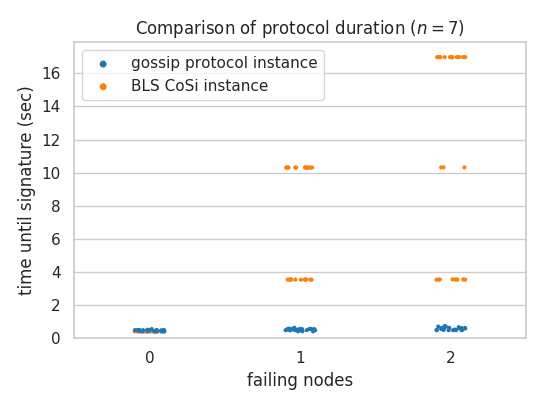
\includegraphics[width=\textwidth]{figures/1/round_wall_sum_7.png}
        \captionsetup{labelformat=empty}
        \caption{Protocol duration, $n = 7$}
    \end{minipage}\hfill
    \begin{minipage}{0.5\textwidth}
        \centering
        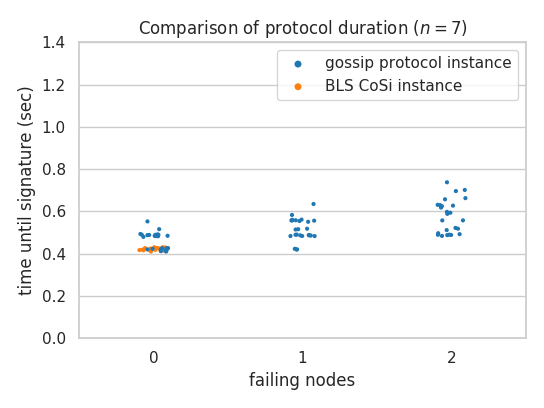
\includegraphics[width=\textwidth]{figures/1/round_wall_sum_zoomed_7.png}
        \captionsetup{labelformat=empty}
        \caption{Protocol duration, $n = 7$, zoomed in to show short instances}
    \end{minipage}\hfill
\end{figure}

\begin{figure}[H]
    \centering
    \begin{minipage}{0.5\textwidth}
        \centering
        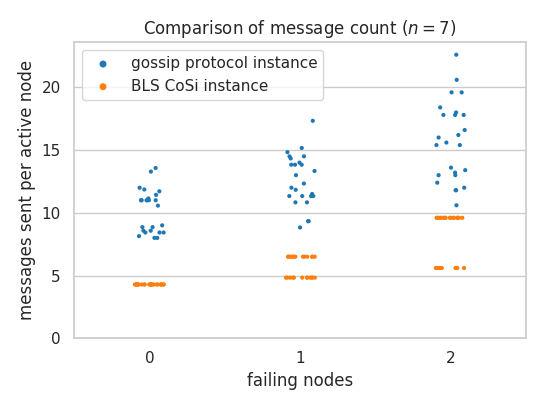
\includegraphics[width=\textwidth]{figures/1/bandwidth_msg_tx_sum_7.png}
        \captionsetup{labelformat=empty}
        \caption{Message count, $n = 7$}
    \end{minipage}\hfill
    \begin{minipage}{0.5\textwidth}
        \centering
        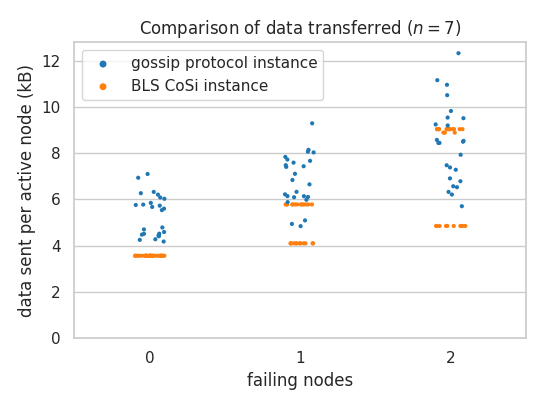
\includegraphics[width=\textwidth]{figures/1/bandwidth_tx_sum_7.png}
        \captionsetup{labelformat=empty}
        \caption{Data transferred, $n = 7$}
    \end{minipage}\hfill
\end{figure}

\begin{figure}[H]
    \centering
    \begin{minipage}{0.5\textwidth}
        \centering
        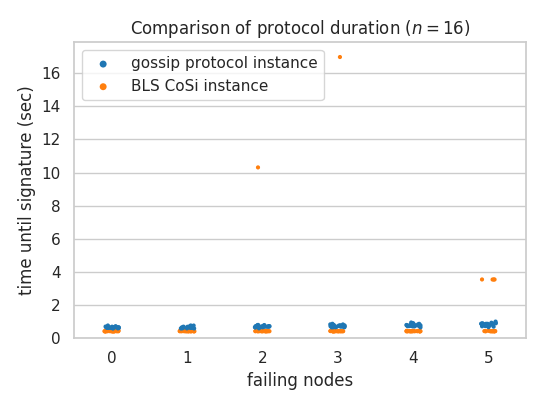
\includegraphics[width=\textwidth]{figures/1/round_wall_sum_16.png}
        \captionsetup{labelformat=empty}
        \caption{Protocol duration, $n = 16$}
    \end{minipage}\hfill
    \begin{minipage}{0.5\textwidth}
        \centering
        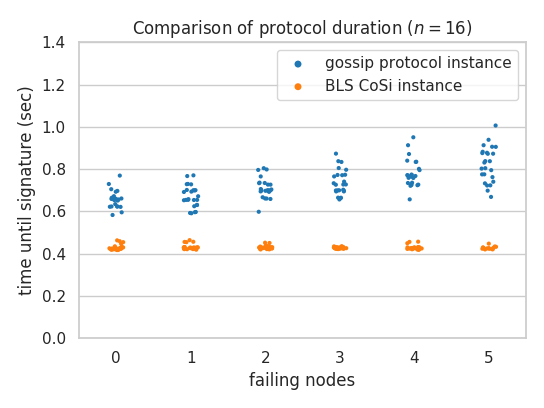
\includegraphics[width=\textwidth]{figures/1/round_wall_sum_zoomed_16.png}
        \captionsetup{labelformat=empty}
        \caption{Protocol duration, $n = 16$, zoomed in to show short instances}
    \end{minipage}\hfill
\end{figure}

\begin{figure}[H]
    \centering
    \begin{minipage}{0.5\textwidth}
        \centering
        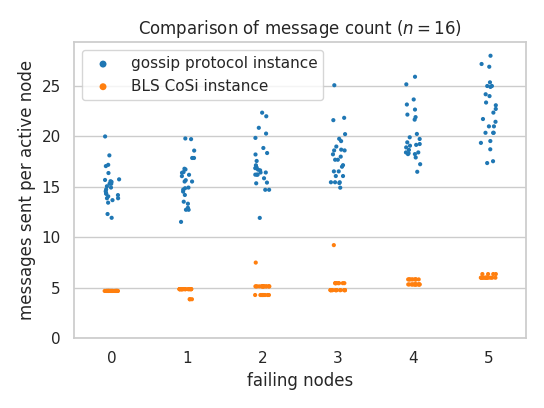
\includegraphics[width=\textwidth]{figures/1/bandwidth_msg_tx_sum_16.png}
        \captionsetup{labelformat=empty}
        \caption{Message count, $n = 16$}
    \end{minipage}\hfill
    \begin{minipage}{0.5\textwidth}
        \centering
        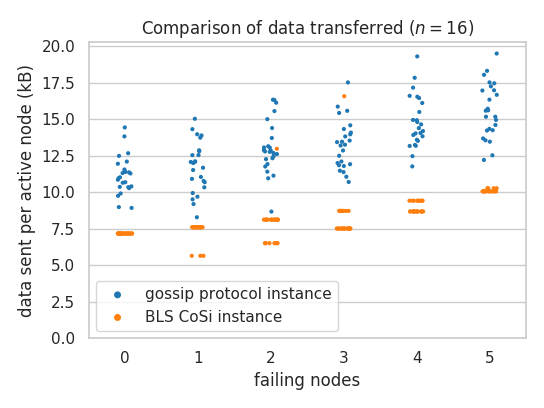
\includegraphics[width=\textwidth]{figures/1/bandwidth_tx_sum_16.png}
        \captionsetup{labelformat=empty}
        \caption{Data transferred, $n = 16$}
    \end{minipage}\hfill
\end{figure}

\begin{figure}[H]
    \centering
    \begin{minipage}{0.5\textwidth}
        \centering
        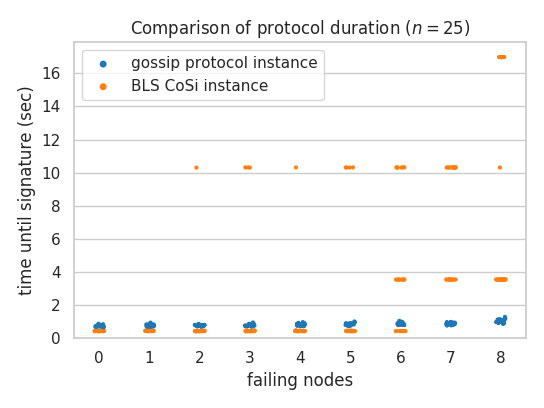
\includegraphics[width=\textwidth]{figures/1/round_wall_sum_25.png}
        \captionsetup{labelformat=empty}
        \caption{Protocol duration, $n = 25$}
    \end{minipage}\hfill
    \begin{minipage}{0.5\textwidth}
        \centering
        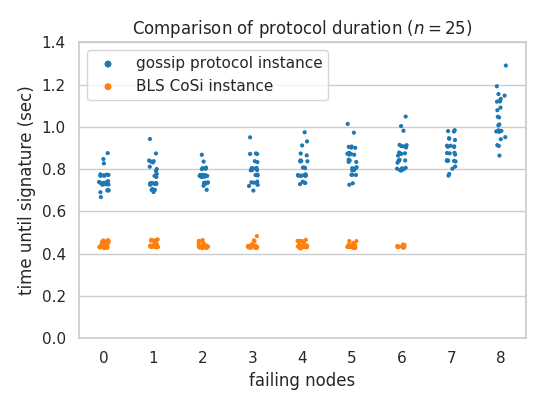
\includegraphics[width=\textwidth]{figures/1/round_wall_sum_zoomed_25.png}
        \captionsetup{labelformat=empty}
        \caption{Protocol duration, $n = 25$, zoomed in to show short instances}
    \end{minipage}\hfill
\end{figure}

\begin{figure}[H]
    \centering
    \begin{minipage}{0.5\textwidth}
        \centering
        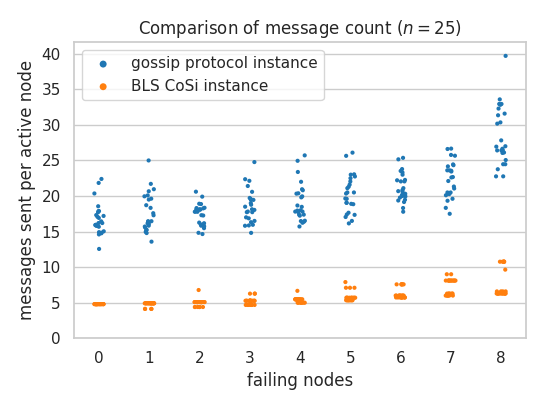
\includegraphics[width=\textwidth]{figures/1/bandwidth_msg_tx_sum_25.png}
        \captionsetup{labelformat=empty}
        \caption{Message count, $n = 25$}
    \end{minipage}\hfill
    \begin{minipage}{0.5\textwidth}
        \centering
        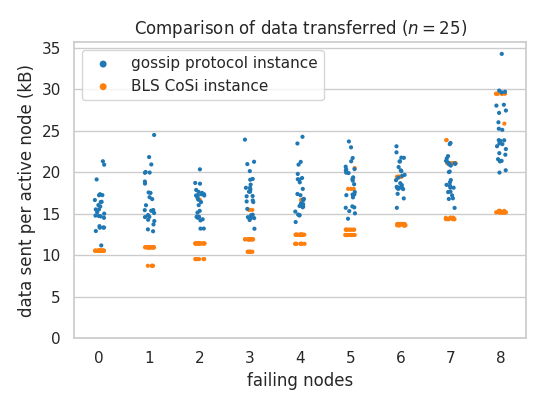
\includegraphics[width=\textwidth]{figures/1/bandwidth_tx_sum_25.png}
        \captionsetup{labelformat=empty}
        \caption{Data transferred, $n = 25$}
    \end{minipage}\hfill
\end{figure}


\begin{figure}[H]
    \centering
    \begin{minipage}{0.5\textwidth}
        \centering
        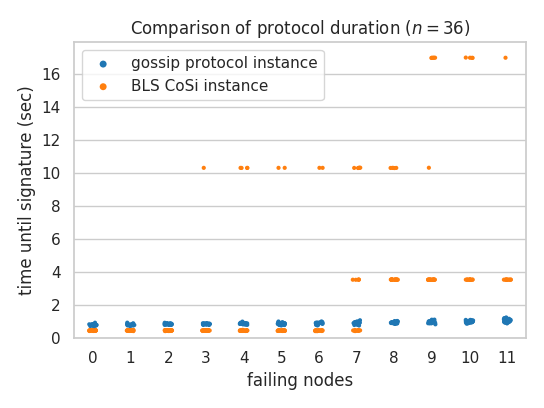
\includegraphics[width=\textwidth]{figures/1/round_wall_sum_36.png}
        \captionsetup{labelformat=empty}
        \caption{Protocol duration, $n = 36$}
    \end{minipage}\hfill
    \begin{minipage}{0.5\textwidth}
        \centering
        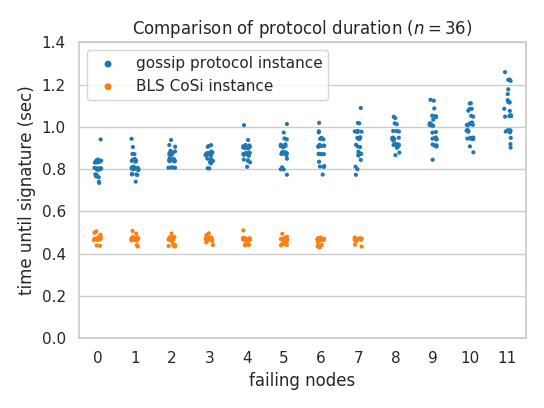
\includegraphics[width=\textwidth]{figures/1/round_wall_sum_zoomed_36.png}
        \captionsetup{labelformat=empty}
        \caption{Protocol duration, $n = 36$, zoomed in to show short instances}
    \end{minipage}\hfill
\end{figure}

\begin{figure}[H]
    \centering
    \begin{minipage}{0.5\textwidth}
        \centering
        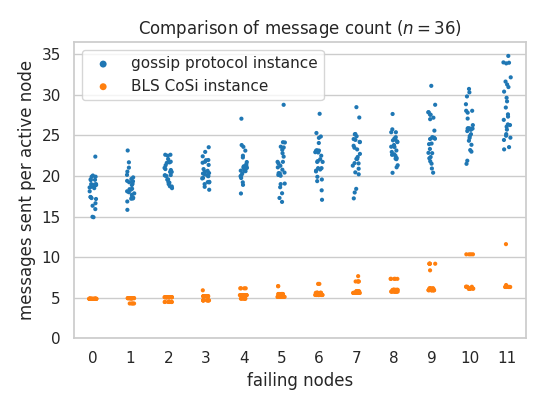
\includegraphics[width=\textwidth]{figures/1/bandwidth_msg_tx_sum_36.png}
        \captionsetup{labelformat=empty}
        \caption{Message count, $n = 36$}
    \end{minipage}\hfill
    \begin{minipage}{0.5\textwidth}
        \centering
        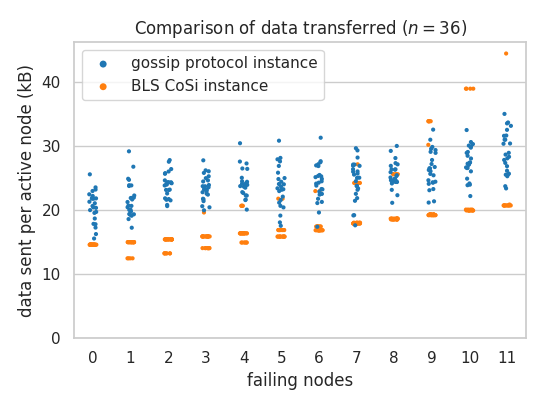
\includegraphics[width=\textwidth]{figures/1/bandwidth_tx_sum_36.png}
        \captionsetup{labelformat=empty}
        \caption{Data transferred, $n = 36$}
    \end{minipage}\hfill
\end{figure}

\begin{figure}[H]
    \centering
    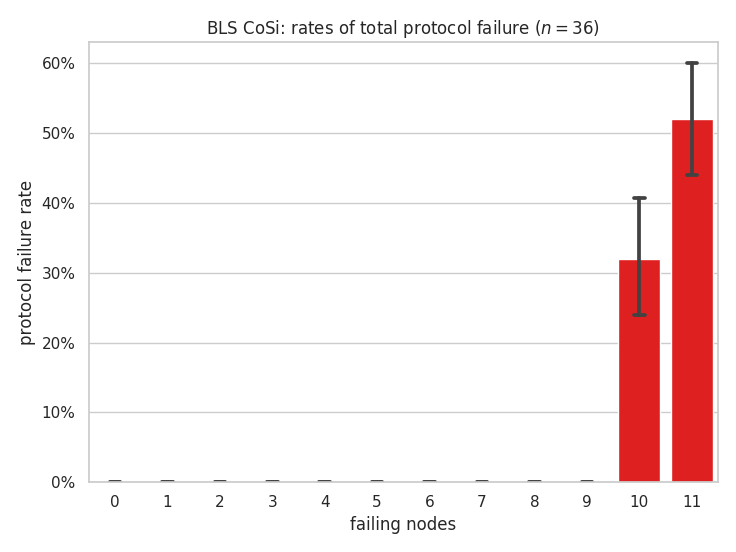
\includegraphics[width=0.95\textwidth]{figures/1/failures_36.png}
    \captionsetup{labelformat=empty}
    \caption{Rates of total protocol failure in BLS CoSi, $n = 36$}
\end{figure}


\newpage
\subsection*{Varying message delay times}

\begin{figure}[H]
    \centering
    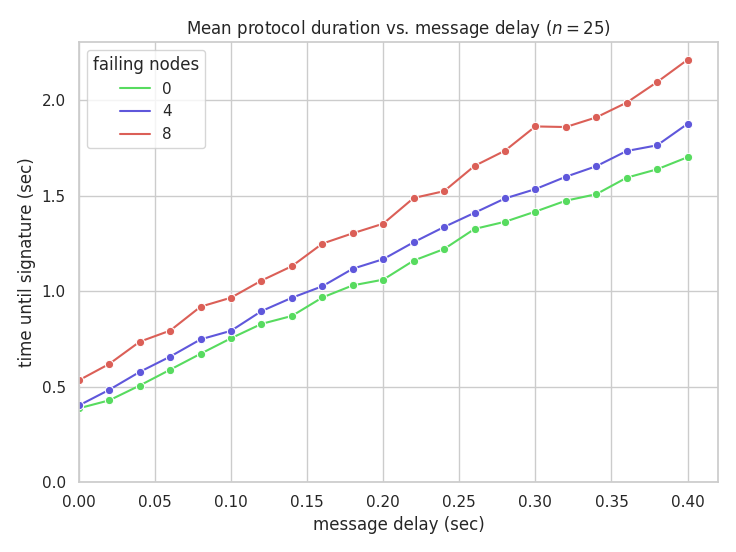
\includegraphics[width=0.95\textwidth]{figures/2/round_wall_sum_by_delay.png}
    \captionsetup{labelformat=empty}
    \caption{Protocol duration vs. mean message delay. The difference between minimum and maximum delay is fixed at 0.01~seconds (except for the special case where the minimum and maximum delay are 0.0~seconds).}
\end{figure}

\begin{figure}[H]
    \centering
    \begin{minipage}{0.5\textwidth}
        \centering
        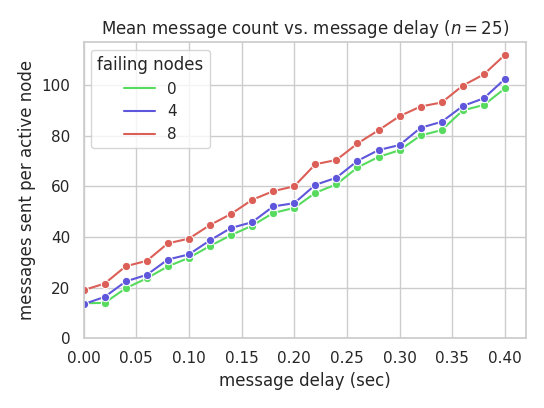
\includegraphics[width=\textwidth]{figures/2/bandwidth_msg_tx_sum_by_delay.png}
        \captionsetup{labelformat=empty}
        \caption{Message count vs. mean message delay}
    \end{minipage}\hfill
    \begin{minipage}{0.5\textwidth}
        \centering
        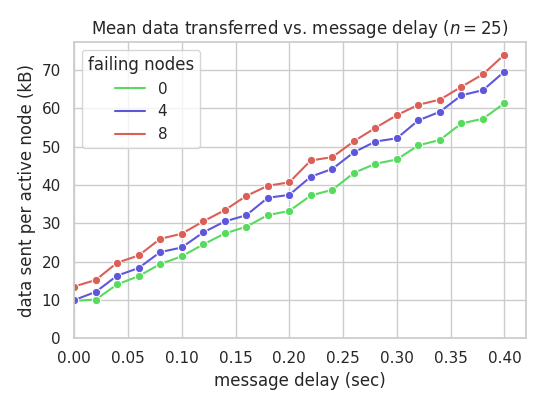
\includegraphics[width=\textwidth]{figures/2/bandwidth_tx_sum_by_delay.png}
        \captionsetup{labelformat=empty}
        \caption{Data transferred vs. mean message delay}
    \end{minipage}\hfill
\end{figure}


\subsection*{Varying numbers of nodes and message delays}

\begin{figure}[H]
    \centering
    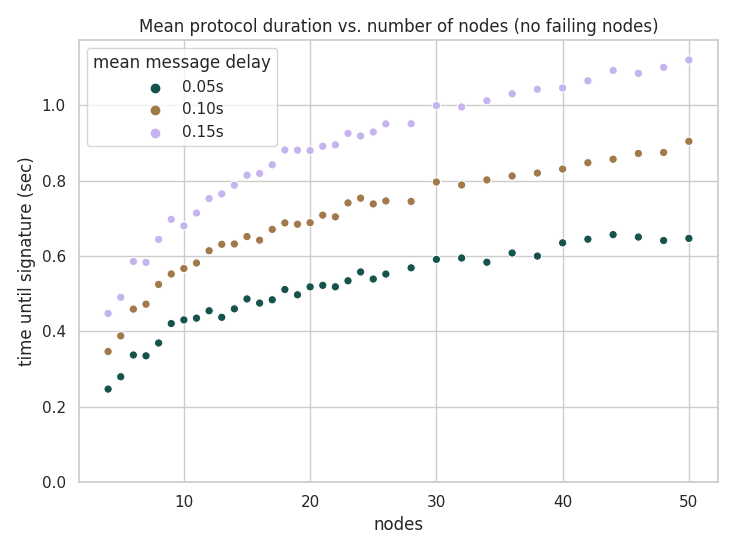
\includegraphics[width=0.95\textwidth]{figures/5/round_wall_sum_by_num_nodes.png}
    \captionsetup{labelformat=empty}
    \caption{Protocol duration vs. number of nodes by mean message delay. The difference between minimum and maximum delay is fixed at 0.01~seconds.}
\end{figure}

\begin{figure}[H]
    \centering
    \begin{minipage}{0.5\textwidth}
        \centering
        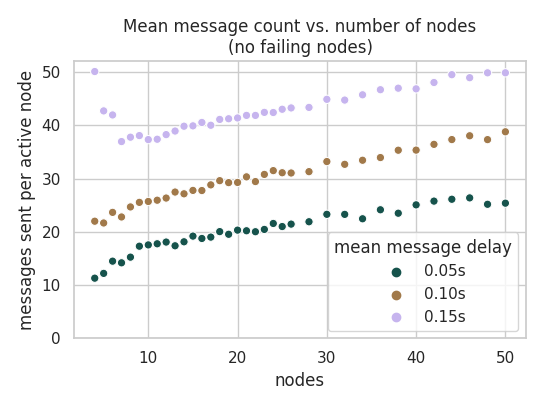
\includegraphics[width=\textwidth]{figures/5/bandwidth_msg_tx_sum_by_num_nodes.png}
        \captionsetup{labelformat=empty}
        \caption{Message count vs. number of nodes by mean message delay}
    \end{minipage}\hfill
    \begin{minipage}{0.5\textwidth}
        \centering
        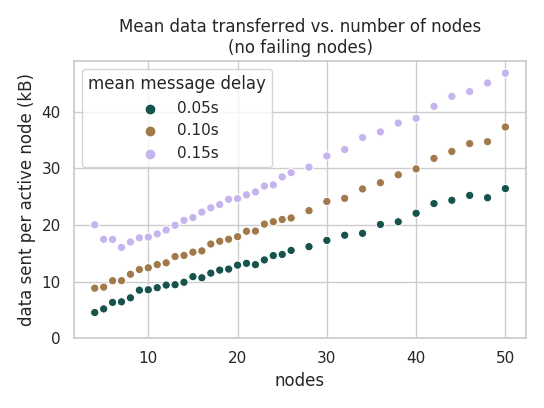
\includegraphics[width=\textwidth]{figures/5/bandwidth_tx_sum_by_num_nodes.png}
        \captionsetup{labelformat=empty}
        \caption{Data transferred vs. number of nodes by mean message delay}
    \end{minipage}\hfill
\end{figure}


\subsection*{Varying numbers of nodes and aggregation settings}

\begin{figure}[H]
    \centering
    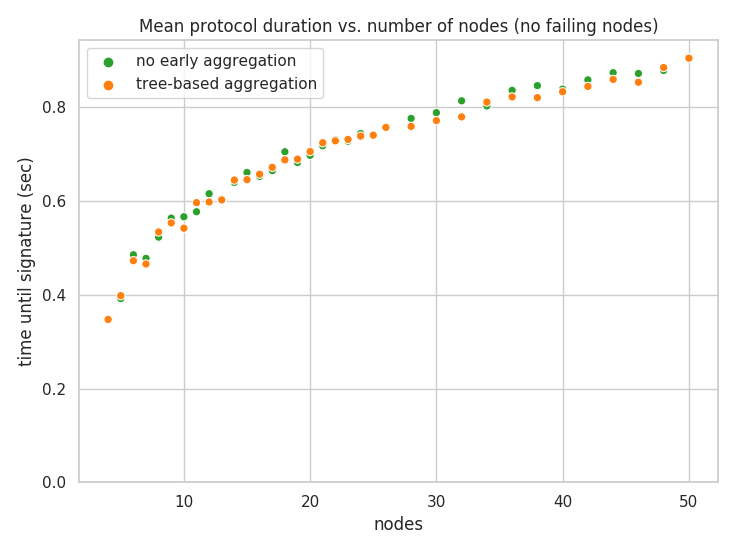
\includegraphics[width=0.95\textwidth]{figures/4/round_wall_sum_by_mode.png}
    \captionsetup{labelformat=empty}
    \caption{Protocol duration vs. number of nodes by aggregation setting}
\end{figure}

\begin{figure}[H]
    \centering
    \begin{minipage}{0.5\textwidth}
        \centering
        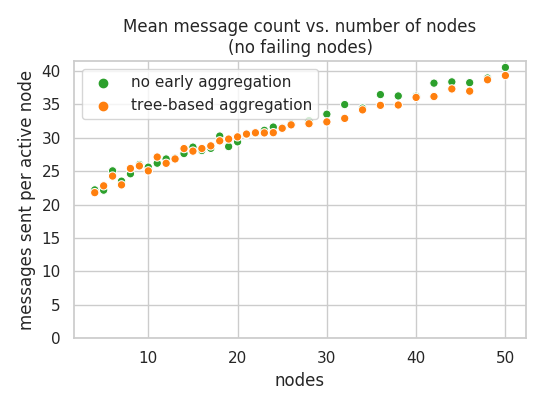
\includegraphics[width=\textwidth]{figures/4/bandwidth_msg_tx_sum_by_mode.png}
        \captionsetup{labelformat=empty}
        \caption{Message count vs. number of nodes by aggregation setting}
    \end{minipage}\hfill
    \begin{minipage}{0.5\textwidth}
        \centering
        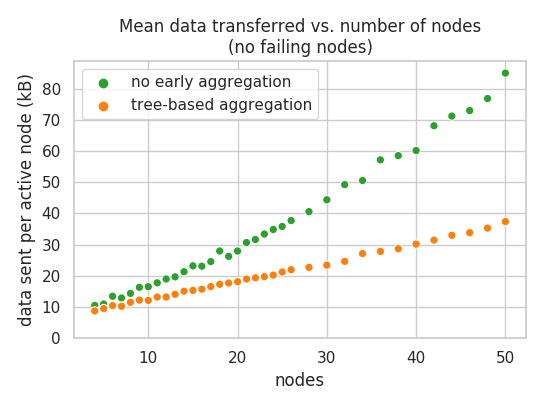
\includegraphics[width=\textwidth]{figures/4/bandwidth_tx_sum_by_mode.png}
        \captionsetup{labelformat=empty}
        \caption{Data transferred vs. number of nodes by aggregation setting}
    \end{minipage}\hfill
\end{figure}


\subsection*{Varying rumor-sending intervals}

\begin{figure}[H]
    \centering
    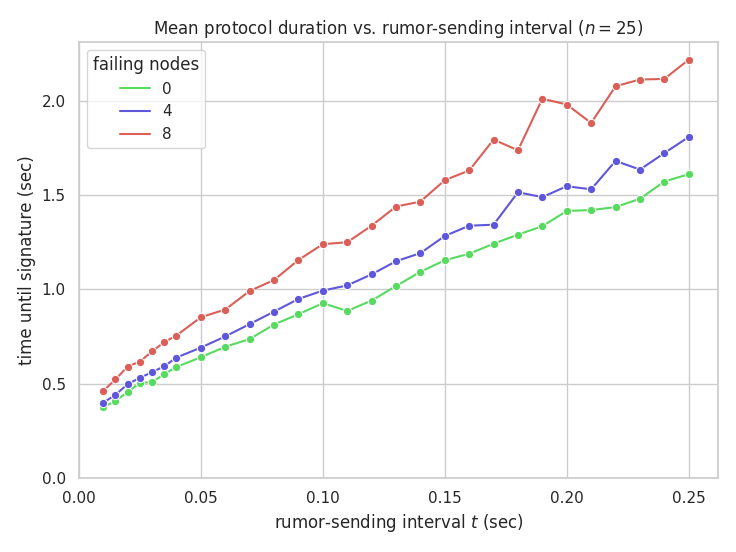
\includegraphics[width=0.95\textwidth]{figures/6/round_wall_sum_by_gossip_tick.png}
    \captionsetup{labelformat=empty}
    \caption{Protocol duration vs. rumor-sending interval $t$}
\end{figure}

\begin{figure}[H]
    \centering
    \begin{minipage}{0.5\textwidth}
        \centering
        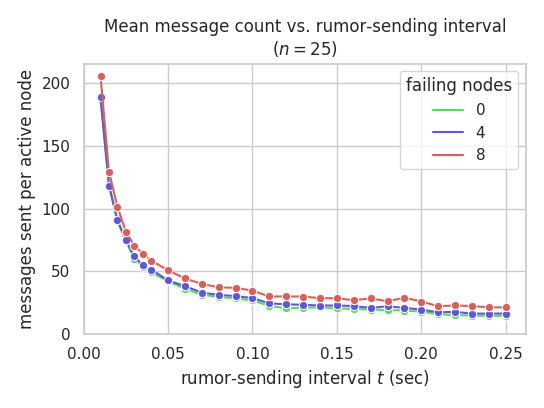
\includegraphics[width=\textwidth]{figures/6/bandwidth_msg_tx_sum_by_gossip_tick.png}
        \captionsetup{labelformat=empty}
        \caption{Message count vs. rumor-sending interval $t$}
    \end{minipage}\hfill
    \begin{minipage}{0.5\textwidth}
        \centering
        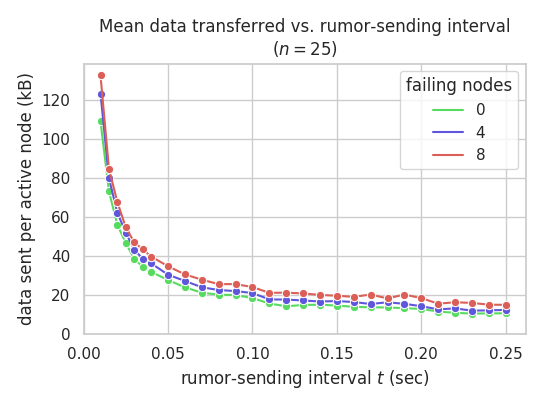
\includegraphics[width=\textwidth]{figures/6/bandwidth_tx_sum_by_gossip_tick.png}
        \captionsetup{labelformat=empty}
        \caption{Data transferred vs. rumor-sending interval $t$}
    \end{minipage}\hfill
\end{figure}


\subsection*{Varying numbers of failing nodes}

\begin{figure}[H]
    \centering
    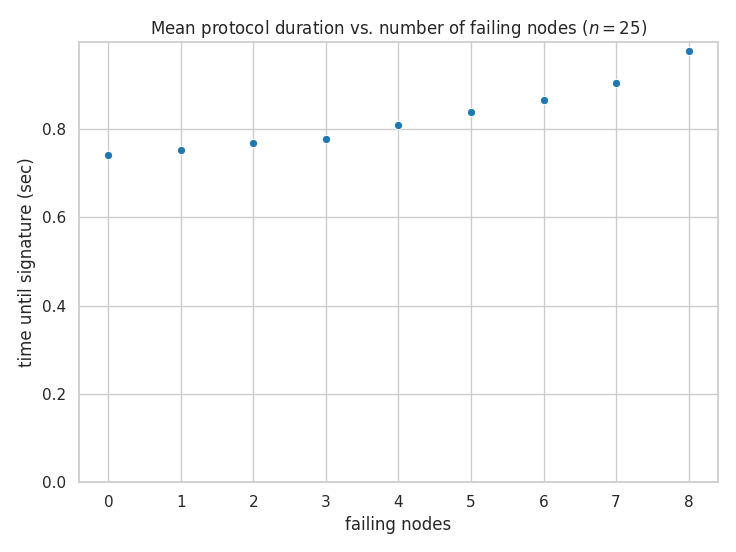
\includegraphics[width=0.95\textwidth]{figures/3/round_wall_sum_by_failing.png}
    \captionsetup{labelformat=empty}
    \caption{Protocol duration vs. number of failing nodes}
\end{figure}

\begin{figure}[H]
    \centering
    \begin{minipage}{0.5\textwidth}
        \centering
        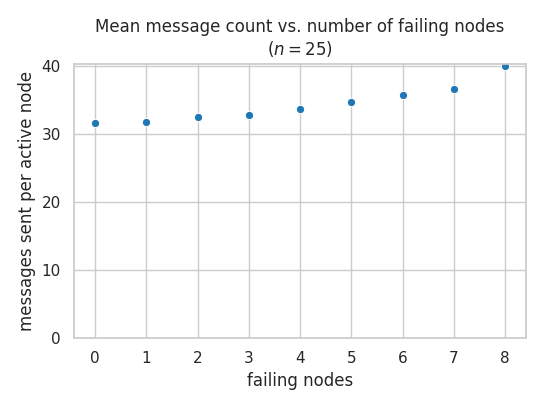
\includegraphics[width=\textwidth]{figures/3/bandwidth_msg_tx_sum_by_failing.png}
        \captionsetup{labelformat=empty}
        \caption{Message count vs. number of failing nodes}
    \end{minipage}\hfill
    \begin{minipage}{0.5\textwidth}
        \centering
        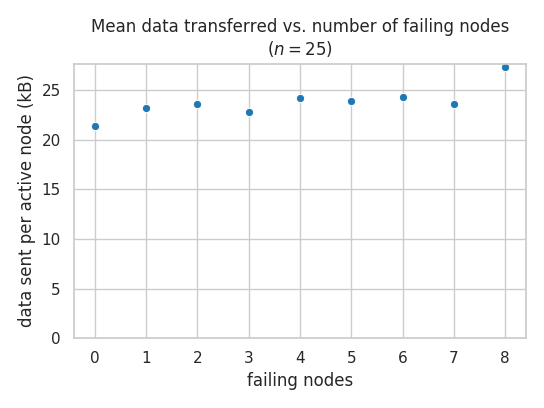
\includegraphics[width=\textwidth]{figures/3/bandwidth_tx_sum_by_failing.png}
        \captionsetup{labelformat=empty}
        \caption{Data transferred vs. number of failing nodes}
    \end{minipage}\hfill
\end{figure}


\subsection*{Varying numbers of rumor-message recipients}

\begin{figure}[H]
    \centering
    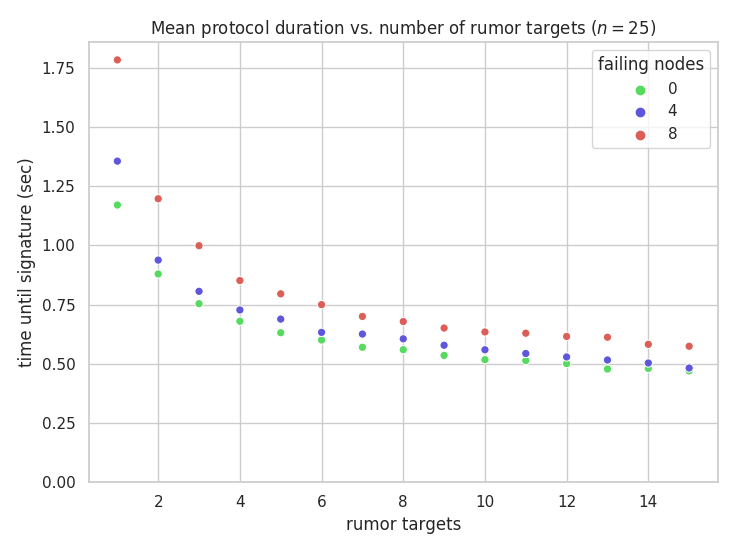
\includegraphics[width=0.95\textwidth]{figures/7/round_wall_sum_by_rumor_targets.png}
    \captionsetup{labelformat=empty}
    \caption{Protocol duration vs. number of rumor targets}
\end{figure}

\begin{figure}[H]
    \centering
    \begin{minipage}{0.5\textwidth}
        \centering
        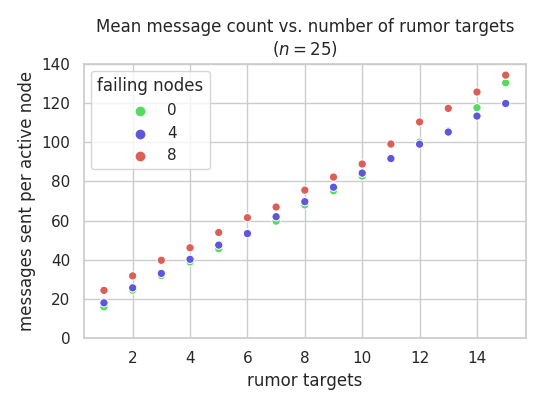
\includegraphics[width=\textwidth]{figures/7/bandwidth_msg_tx_sum_by_rumor_targets.png}
        \captionsetup{labelformat=empty}
        \caption{Message count vs. number of rumor targets}
    \end{minipage}\hfill
    \begin{minipage}{0.5\textwidth}
        \centering
        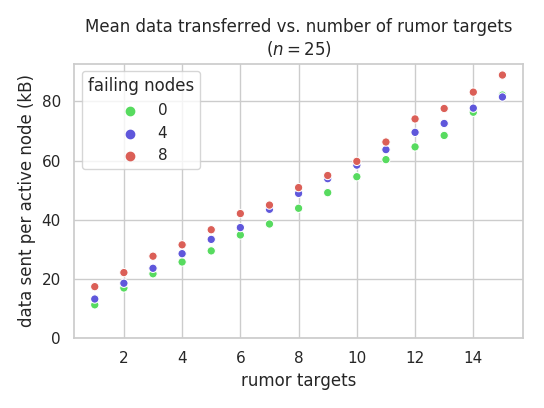
\includegraphics[width=\textwidth]{figures/7/bandwidth_tx_sum_by_rumor_targets.png}
        \captionsetup{labelformat=empty}
        \caption{Data transferred vs. number of rumor targets}
    \end{minipage}\hfill
\end{figure}


\subsection*{Varying numbers of shutdown-message recipients}

\begin{figure}[H]
    \centering
    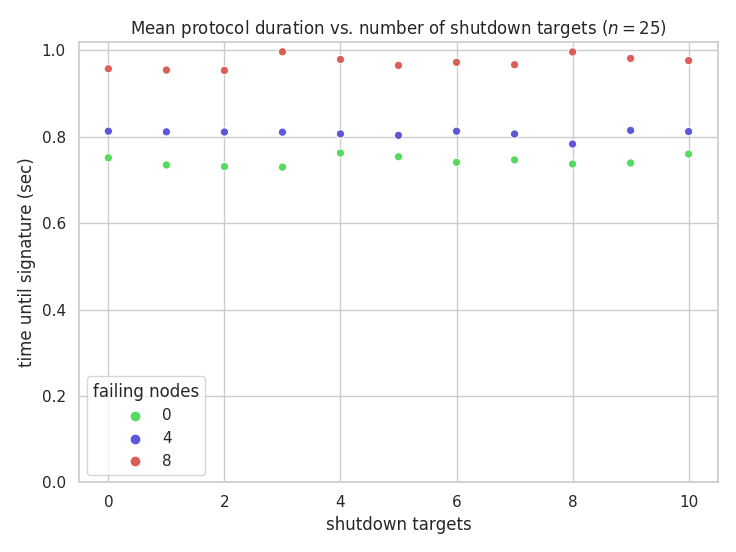
\includegraphics[width=0.95\textwidth]{figures/8/round_wall_sum_by_shutdown_targets.png}
    \captionsetup{labelformat=empty}
    \caption{Protocol duration vs. number of shutdown targets}
\end{figure}

\begin{figure}[H]
    \centering
    \begin{minipage}{0.5\textwidth}
        \centering
        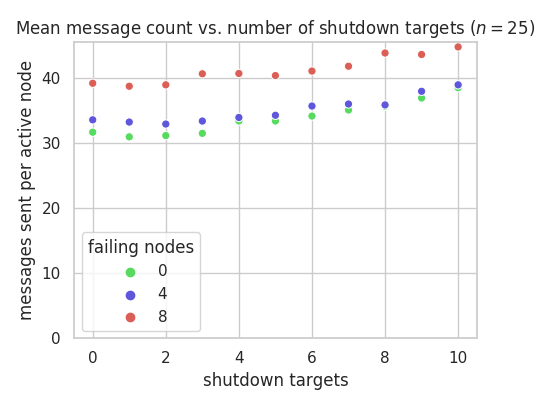
\includegraphics[width=\textwidth]{figures/8/bandwidth_msg_tx_sum_by_shutdown_targets.png}
        \captionsetup{labelformat=empty}
        \caption{Message count vs. number of shutdown targets}
    \end{minipage}\hfill
    \begin{minipage}{0.5\textwidth}
        \centering
        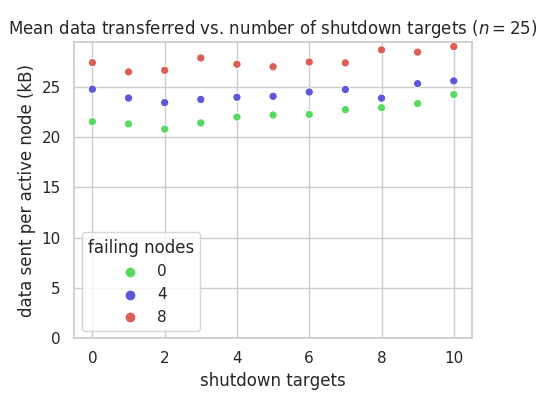
\includegraphics[width=\textwidth]{figures/8/bandwidth_tx_sum_by_shutdown_targets.png}
        \captionsetup{labelformat=empty}
        \caption{Data transferred vs. number of shutdown targets}
    \end{minipage}\hfill
\end{figure}


\subsection*{Varying numbers of rumor-message recipients, rumor-sending interval adjusted}

\begin{figure}[H]
    \centering
    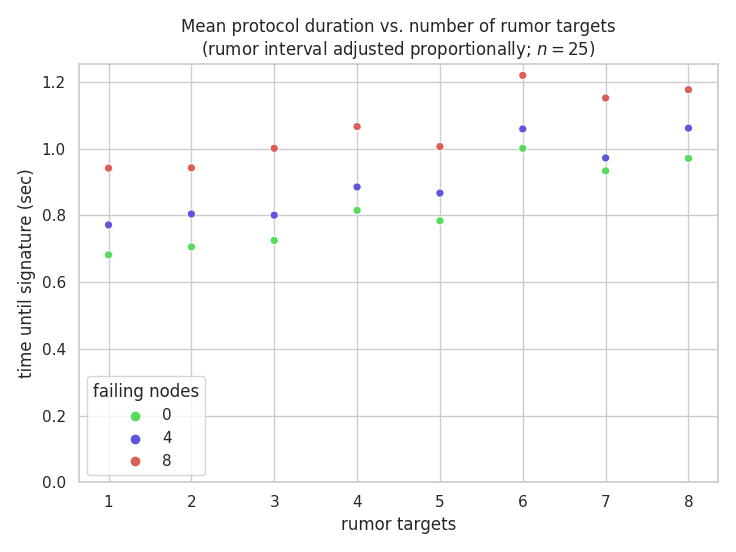
\includegraphics[width=0.95\textwidth]{figures/9/round_wall_sum_by_rumor_targets.png}
    \captionsetup{labelformat=empty}
    \caption{Protocol duration vs. number of rumor targets. The rumor-sending interval $t$ is adjusted proportionally to the number of rumor targets so that the number of messages sent per node per second is always 42.9.}
\end{figure}

\begin{figure}[H]
    \centering
    \begin{minipage}{0.5\textwidth}
        \centering
        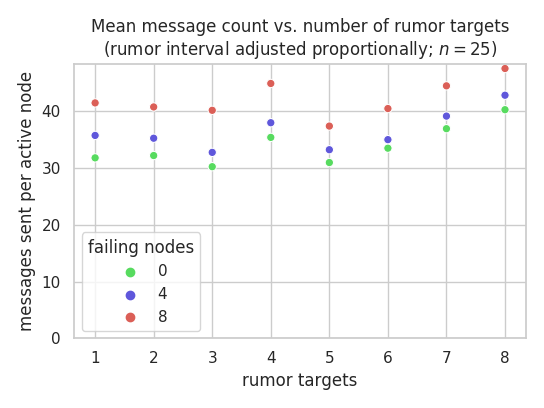
\includegraphics[width=\textwidth]{figures/9/bandwidth_msg_tx_sum_by_rumor_targets.png}
        \captionsetup{labelformat=empty}
        \caption{Message count vs. number of rumor targets. The rumor-sending interval $t$ is adjusted proportionally.}
    \end{minipage}\hfill
    \begin{minipage}{0.5\textwidth}
        \centering
        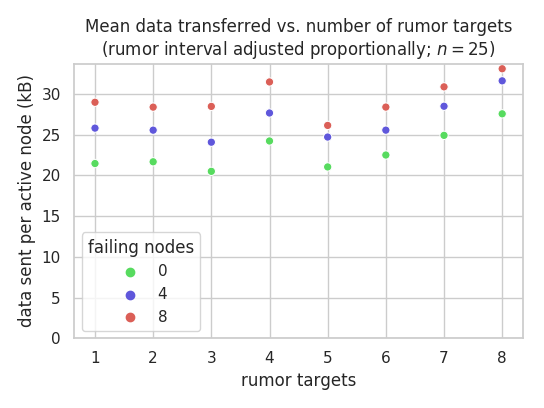
\includegraphics[width=\textwidth]{figures/9/bandwidth_tx_sum_by_rumor_targets.png}
        \captionsetup{labelformat=empty}
        \caption{Data transferred vs. number of rumor targets. The rumor-sending interval $t$ is adjusted proportionally.}
    \end{minipage}\hfill
\end{figure}


\subsection*{Varying message delay variance}

\begin{figure}[H]
    \centering
    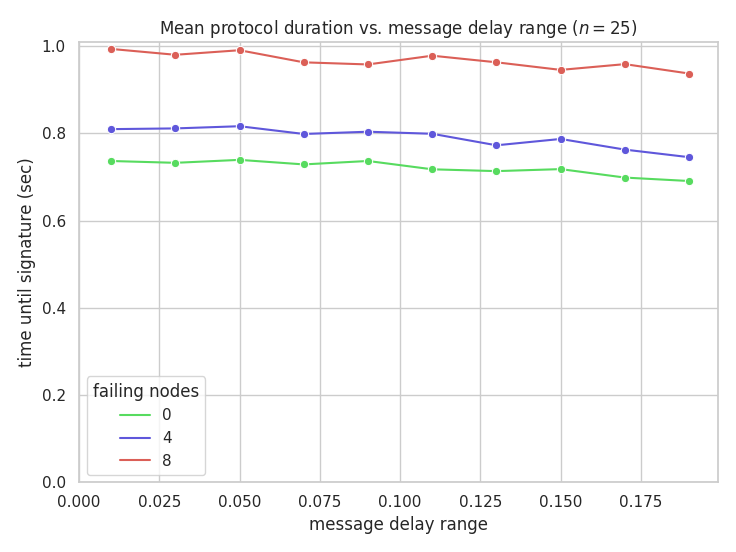
\includegraphics[width=0.95\textwidth]{figures/10/round_wall_sum_by_delay_range.png}
    \captionsetup{labelformat=empty}
    \caption{Protocol duration vs. the difference between the minimum and maximum message delay. The mean message delay is fixed at 0.1~seconds.}
\end{figure}

\begin{figure}[H]
    \centering
    \begin{minipage}{0.5\textwidth}
        \centering
        \includegraphics[width=\textwidth]{figures/10/bandwidth_msg_tx_sum_by_delay_range.png}
        \captionsetup{labelformat=empty}
        \caption{Message count vs. the difference between the minimum and maximum message delay}
    \end{minipage}\hfill
    \begin{minipage}{0.5\textwidth}
        \centering
        \includegraphics[width=\textwidth]{figures/10/bandwidth_tx_sum_by_delay_range.png}
        \captionsetup{labelformat=empty}
        \caption{Data transferred vs. the difference between the minimum and maximum message delay}
    \end{minipage}\hfill
\end{figure}


\newpage
\raggedright
\bibliographystyle{unsrt}
\bibliography{references}
\addcontentsline{toc}{section}{References}
